\documentclass[slidestop,compress,mathserif]{beamer}
\usepackage[bars]{beamerthemetree} % Beamer theme v 2.2
\usetheme{Madrid} % Beamer theme v 3.0
\usecolortheme{seagull} % Beamer color theme
\usepackage{bibentry}
\usepackage{graphicx}
\usepackage{epigraph}
\usepackage{makeidx}
\makeindex
\usepackage[]{amsmath}
\usepackage[]{amssymb}
\usepackage{color}
\usepackage{pict2e}
\usepackage{algorithm2e}
\usepackage[ngerman]{babel}
\usepackage{tikz}
\usepackage[europeanresistors,europeaninductors]{circuitikz}
\usepackage{multirow}
\usepackage[utf8]{inputenc}
\usepackage{multimedia}
\usepackage{xcolor}
\usetikzlibrary{arrows, decorations.markings}
\tikzstyle{vecArrow} = [thick, decoration={markings,mark=at position
   1 with {\arrow[semithick]{open triangle 60}}},
   double distance=1.4pt, shorten >= 5.5pt,
   preaction = {decorate},
   postaction = {draw,line width=1.4pt, white,shorten >= 4.5pt}]
\tikzstyle{innerWhite} = [semithick, white,line width=1.4pt, shorten >= 4.5pt]



\definecolor{blue}{rgb}{0,0,1}
\definecolor{mint}{cmyk}{75,0,40,0}
\definecolor{mint}{rgb}{32,178,170}
\begin{document}
% Formalia
\newcommand{\revision}{Rev. D}
\newcommand{\docnum}{SFV-14031}
\newcommand{\done}{${\color{teal}\checkmark}$}
\newcommand{\Var}{\operatorname{Var}}
\newcommand{\D}{\operatorname{d}}
\newcommand{\mum}{\operatorname{\mu m}}
\newcommand{\E}{\operatorname{E}}
\newcommand{\var}{\operatorname{var}}
\newcommand{\Id}{\operatorname{Id}}
\newcommand{\rg}{\operatorname{rg}}

\newcommand{\offslide}[2]{\frame{\frametitle{ 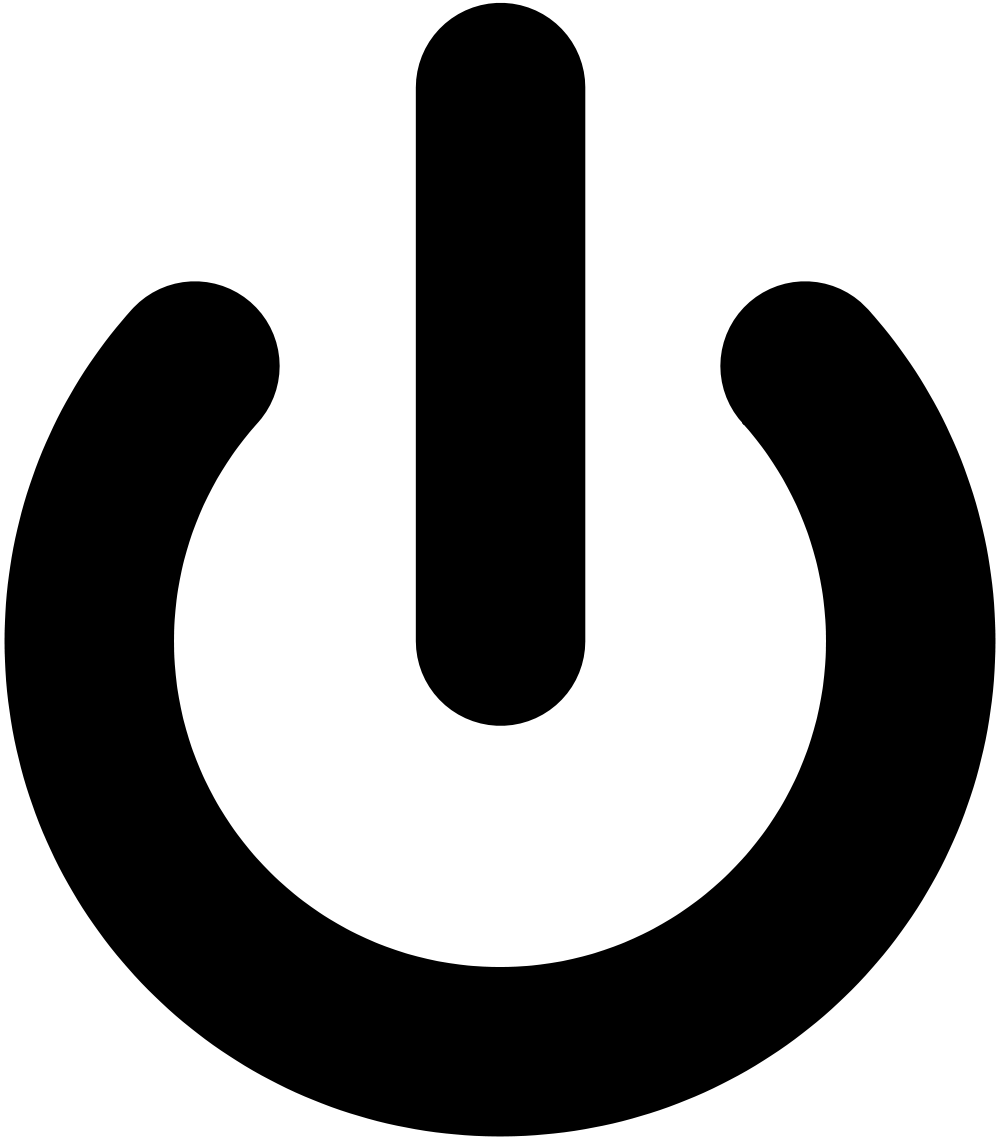
\includegraphics[scale=0.01] {Off}\hspace{1.5mm} #1}
\framesubtitle{#2}
}}
\newcommand{\source}[1]{\rotatebox{90}{\tiny \color{gray} #1}}


%\newtheorem{lemma}{Lemma}
\title{85741: Energieeffiziente Antriebsregelungen}
%\date{}
\subtitle{Regelung im Zustandsraum}
\author[R. Pfaff]{Prof. Dr. Raphael Pfaff}
\institute[Dokument \docnum, \revision]{Fachhochschule Aachen}
\logo{\put(-362, 0){
\includegraphics[width=0.5cm]{logo.jpg}}}

\begin{frame} % Cover slide
\titlepage
\end{frame}

\frame{\frametitle{Lernziele}
\framesubtitle{}
\begin{itemize}
\item Teil 1:
\begin{itemize}
	\scriptsize
		\item Die Studierenden kennen die Zustandsraumbeschreibung, die Bedeutung von Polstellen und die Begriffe Steuerbarkeit und Beobachtbarkeit.
		\item Die Studierenden kennen die Normalformen der Zustandsbeschreibung und zugeh\"orige Blockdiagramme.
		\item Die Studierenden kennt die Blockdiagramme und resultierenden Systemmatrizen der Regelung im Zustandsraum sowie den Unterschied zwischen Zustands- und Ausgangsr\"uckf\"uhrung.
		\end{itemize}
		\item Teil 2:
		\begin{itemize}
		\scriptsize
		\item Die Studierenden kennen Sch\"atzfunktionen und deren w\"unschenswerte Eigenschaften.
		\item Die Studierenden kennen den grunds\"atzlichen Aufbau der Prediction Error Methods (PEM) und ihre Eigenschaften.
		\item Die Studierenden k\"onnen den Kalman Filter als Zustandssch\"atzer sowie den RLS a\"ls Parametersch\"atzer anwenden und ihre Grenzen aufzeigen.
		\end{itemize}
		\item Teil 3 (Rechnerpraktikum/Selbststudium):
		\begin{itemize}
		\scriptsize
		\item Die Studierenden k\"onnen dynamische Systeme im Zustandsraum simulieren.
		\item Die Studierenden k\"onnen Zustands- und Parametersch\"atzer in Scicos oder C implementieren.
		\end{itemize}
\end{itemize}
}

\frame{\frametitle{Struktur des Kurses}
\framesubtitle{}
\begin{center}
            		\begin{tikzpicture}[thick]
		%\tiny
  \node[draw,rectangle] (a) {Zustandsraumbeschreibung};
  \node[draw,rectangle,below of=a, left of = a, anchor = east] (b) {Modellierung};
  \node[draw,rectangle,below of=b] (c) {Parameter};
\node[draw,rectangle,below of=c] (d) {Normalformen};
\node[draw,rectangle,below of=d] (e) {Matrixexponential};
 
 
  \node[draw,rectangle,below of=a, right of = a, anchor = west] (g) {Regelung};
  \node[draw,rectangle,below of=g] (h) {R\"uckf\"uhrung};
  \node[draw,rectangle,below of=h] (i) {MPC};
  \node[draw,rectangle,below of=i] (j) {Beobachter};
  \node[draw,rectangle,below of=j] (k) {Kalman Filter};
\node[draw,rectangle,below of=k, anchor = east] (f) {Regelung im Zustandsraum};

  \draw[->] (a) |- (b);
  \draw[->] (b) -- (c);
  \draw[->] (c) -- (d);
  \draw[->] (d) -- (e); 
  \draw[->] (e) -| (f);
  
  \draw[->] (a) |- (g);
  \draw[->] (g) -- (h);
  \draw[->] (h) -- (i);
  \draw[->] (i) -- (j); 
  \draw[->] (j) -- (k);
  \draw[->] (k) -| (f);
  
  
\end{tikzpicture}
\end{center}
}

\section{Einf\"uhrung Zustandsraum}
\frame{\sectionpage}
\frame{\frametitle{Einf\"uhrung Zustandsraum \textit{(state space)}}
\framesubtitle{Der Zustandsraum ist eine zunehmend an Bedeutung gewinnende Darstellung eines dynamischen Systems.}
\begin{columns}[t] 
     \begin{column}[T]{6cm} 
     	\begin{itemize}
     		\item Zustandsvariablen $x_{i}(t)$:
		\begin{itemize}
		\item Energiegehalt der Speichersysteme
		\item Bilden Zustandsvektor $x(t)$
		\end{itemize}
		\item $x(t_{0})$ enth\"alt alle Informationen \"uber System zum Zeitpunkt $t_{0}$
		\item \"Uberf\"uhrung der DGL $n$-ter Ordnung in $n$ DGL 1. Ordnung
		\item Hier betrachtet: \textit{single-input-single-output} (SISO) System
     	\end{itemize}
     \end{column}
     	\begin{column}[T]{6cm} 
		\textbf{Zustandsraumdarstellung:}
         	\begin{block}{Zeitkontinuierlich}
		\begin{eqnarray}
			\dot{x}(t) &= A x(t) + B u(t) \label{Eq:SSCT1}\\
			y(t) &= Cx(t) + D u(t) \label{Eq:SSCT2}
		\end{eqnarray}
		\end{block}
		\begin{block}{Zeitdiskret}
         	\begin{eqnarray}
			x_{k+1} &= A x_{k} + B u_{k} \label{Eq:SSDT1}\\
			y_{k} &= Cx_{k} + D u_{k} \label{Eq:SSDT2}
		\end{eqnarray}
		\end{block}
     \end{column}
 \end{columns}
}

\frame{\frametitle{Bedeutung der Variablen und Parameter}
\framesubtitle{Gr\"o{\ss}en der Variablen und Parameter f\"ur SISO System der Ordnung $n$, $\cdot(t)$ beschreibt Variablen, d.h. $\cdot_{k}$ bzw. $\cdot(t)$.}
\begin{columns}[t] 
     \begin{column}[T]{6cm} 
     	\begin{itemize}
     		\item $A \in \mathbb{R}^{n \times n}$: Systemmatrix
		\begin{itemize}
		\item Systeminformationen, z.B. Polstellen, Beobachtbarkeit, ...
		\end{itemize}
		\item $B \in \mathbb{R}^{n \times 1}$: Eingangsvektor
		\begin{itemize}
		\item Wirkung von $u$ auf System
		\end{itemize}
		\item $C \in \mathbb{R}^{1 \times n}$: Ausgangsvektor
		\begin{itemize}
		\item Wirkung von $x$ auf Ausgang
		\end{itemize}
		\item $D \in \mathbb{R}$: Feedforward term
		\begin{itemize}
		\item Direkte Wirkung von $u$ auf Ausgang
		\end{itemize}
     	\end{itemize}
     \end{column}
     	\begin{column}[T]{6cm} 
         	\begin{eqnarray*}
			\dot{x}(t) &= A x(t) + B u(t) \\
			y(t) &= Cx(t) + D u(t) \\ \vspace{.5cm}
			x_{k+1} &= A x_{k} + B u_{k} \\
			y_{k} &= Cx_{k} + D u_{k}
		\end{eqnarray*}
		\begin{itemize}
		\item $x(t) \in \mathbb{R}^{n \times 1}$: Zustandsvektor
		\begin{itemize}
		\item Zustand der Energiespeicher
		\end{itemize}
		\item $u(t) \in \mathbb{R}$: Eingangswert in System
		\item $y(t) \in \mathbb{R}$: Ausgangswert des Systems
		\end{itemize}
     \end{column}
 \end{columns}
}

\offslide{Erarbeitung konzeptionelles Blockdiagramm}

\frame{\frametitle{Vorteile/Nachteile Zustandsraumdarstellung}
\framesubtitle{}
\begin{itemize}
\item[+] Reichhaltige Beschreibung: interne Werte des Systems werden modelliert
\item[+] Vollst\"andige Abbildung des Systemzustands durch die $x_{i}$
\item[+] Digitale Regler im Zustandsraum performanter
\item[+] F\"ur Energieeffizienz: Energiegehalt des System wird modelliert
\item[+] Zustand hat h\"aufig physikalische Bedeutung
\item[-] Zustandsraumdarstellung nicht eindeutig
\item[-] Teils numerisch/analytisch aufwendig
\end{itemize}
}


\frame{\frametitle{Zustandsraumdarstellung RLC-System}
\framesubtitle{}
         \begin{center}
		\begin{circuitikz}[scale = 0.8]
		\draw 
	(-2,0) to  [V=$u(t)$] (-2,4)
		to [R=$R$,  i>^=$i(t)$] (2,4)
		to [L=$L$] (6,4)
		to [C=$C$, v_>=$u_{C}(t)$] (6,0)
  		 to [short] (-2,0);
		 \end{circuitikz}
        	\end{center}
	\vspace{-1cm}
	\begin{columns}[t] 
     \begin{column}[T]{.5cm} 
     \end{column}
     	\begin{column}[T]{10cm} 
         	\begin{center}
%	\only<1>{
%%	\begin{block}{\"Ubung 1}
%%	Stellen Sie eine Zustandsraumbeschreibung f\"ur den Zustandsvektor $\begin{pmatrix} 
%%		u_{C}(t) \\ \frac{1}{C} i(t)
%%		\end{pmatrix}$ auf.
%%		\end{block}
%	}
%	\only<2>{
	\begin{eqnarray}
		\dot{x}(t) &=& 
		\begin{pmatrix} 
		0 & 1 \\ \frac{-1}{L C} & \frac{-R}{L}
		\end{pmatrix}
		\begin{pmatrix} 
		x_{1}(t) \\ x_{2}(t)
		\end{pmatrix} +
		\begin{pmatrix} 
		0 \\ \frac{1}{LC} 
		\end{pmatrix} u(t) \\
		y(t) &=& u_{C}(t) = \begin{pmatrix} 
		1 & 0
		\end{pmatrix}
		 \begin{pmatrix} 
		x_{1}(t) \\ x_{2} (t)
		\end{pmatrix}
	\end{eqnarray}
%}
\end{center}
     \end{column}
 \end{columns}
}



\frame{\frametitle{Regelungsnormalform \textit{(control canonical form)}}
	\begin{equation*}
		\begin{split}
		&\frac{\D^{n} y}{\D t^{n}} + a_{n-1} \frac{\D^{n-1} y}{\D t^{n-1}} + \cdots + a_{1} \frac{\D y}{\D t} + a_{0} y  \\
		&= b_{n} \frac{\D^{n} u}{\D t^{n}} + b_{n-1} \frac{\D^{n-1} u}{\D t^{n-1}} + \cdots + b_{1} \frac{\D u}{\D t} + b_{0} u 
		\end{split}
	\end{equation*}
\begin{columns}[t] 
     \begin{column}[T]{8cm} 
     	\begin{eqnarray*}
            A&=& \begin{pmatrix}%{ccccc}
             0 & 1  &  0 & \cdots & 0 \\
             0 & 0  &  1 & \cdots & 0 \\
            \vdots &  \vdots &  \vdots & \ddots & \vdots \\
            0 & 0 & 0 & \cdots & 1 \\
            -a_{0} & -a_{1} & -a_{2} &\cdots & -a_{n-1}   
            \end{pmatrix} \\
            C &=& \begin{pmatrix} b_{0} - b_{n}a_{0} & b_{1} - b_{n}a_{1} & \cdots & b_{n-1} - b_{n}a_{n-1} \end{pmatrix}
	\end{eqnarray*}
     \end{column}
     	\begin{column}[T]{3cm} 
         	\begin{eqnarray*}
                 B &=& \begin{pmatrix} 0 \\ 0 \\ \vdots \\ 0 \\ 1\end{pmatrix} \\
                 D &=& b_{n}%\footnote{\"Ublich: $b_{n} = 0$}
	\end{eqnarray*}
     \end{column}
 \end{columns}
}

\offslide{Darstellung Regelungsnormalform im Blockdiagramm}

\frame{\frametitle{Beobachtungsnormalform \textit{(observer canonical form)}}
\begin{equation*}
		\begin{split}
		&\frac{\D^{n} y}{\D t^{n}} + a_{n-1} \frac{\D^{n-1} y}{\D t^{n-1}} + \cdots + a_{1} \frac{\D y}{\D t} + a_{0} y  \\
		&= b_{n} \frac{\D^{n} u}{\D t^{n}} + b_{n-1} \frac{\D^{n-1} u}{\D t^{n-1}} + \cdots + b_{1} \frac{\D u}{\D t} + b_{0} u 
		\end{split}
	\end{equation*}
\begin{columns}[t] 
     \begin{column}[T]{7cm} 
     	\begin{eqnarray*}
            A&=& \begin{pmatrix}%{ccccc}
             0 & \cdots & 0 &  0  & -a_{0} \\
             1 & \cdots & 0  &  0  & -a_{1} \\
            \vdots &  \ddots & \vdots &  \vdots  & \vdots \\
            0 & \cdots & 1 & 0  &  -a_{n-2} \\
            0 & \cdots&  0 & 1  & -a_{n-1}   
            \end{pmatrix} \\
            C &=& \begin{pmatrix} 0 & 0 & \cdots & 0 & 1\end{pmatrix} 
	\end{eqnarray*}
     \end{column}
     	\begin{column}[T]{4cm} 
         	\begin{eqnarray*}
                 B &=&  \begin{pmatrix} b_{0} - b_{n}a_{0} \\ b_{1} - b_{n}a_{1} \\ b_{2} - b_{n}a_{2}\\ \vdots \\ b_{n-1} - b_{n}a_{n-1} \end{pmatrix}\\
                 D &=& b_{n}%\footnote{\"Ublich: $b_{n} = 0$}
	\end{eqnarray*}
     \end{column}
 \end{columns}
}

\offslide{Darstellung Beobachtungsnormalfom im Blockdiagramm}

%\frame{\frametitle{\"Ubung 2: Transformation \"Ubertragungsfunktion in Zustandsraumdarstellung}
%Es sei \[G(s) = \frac{Y(s)}{U(s)} = \frac{s+3}{(s+1)(s+10)}\] die \"Ubertragungsfunktion eines Systems.
%\begin{block}{\"Ubung 2}
%Stellen Sie $G(s)$ dar als:
%\begin{enumerate}
%		\item Differentialgleichung
%		\item Zustandsraumdarstellung f\"ur einen Zustandsvektor $\begin{pmatrix} \dot{x} \\ x\end{pmatrix}$ in
%		\begin{enumerate}
%		\item Regelungsnormalform
%		\item Beobachtungsnormalform
%		\end{enumerate}
%		\end{enumerate}
%\end{block}
%}


\frame{\frametitle{Jordan Normalform \textit{(modal canonical form)}}
	\begin{itemize}
		\item F\"ur System mit Polstellen $\lambda_{i}$
		\item Transferfunktion $G(s) = \sum_{i=1}^{n} \frac{c_{i}}{s-\lambda_{i}} $ 
	\end{itemize}
\begin{columns}[t] 
     \begin{column}[T]{7cm} 
     	\begin{eqnarray*}
            A&=& \begin{pmatrix}%{ccccc}
              \lambda_{1}  &  0 & \cdots & 0 \\
              0  &  \lambda_{2} & \cdots & 0 \\
            \vdots &  \vdots & \ddots & \vdots \\
            0 & 0 &\cdots & \lambda_{n}   
            \end{pmatrix} \\
            C &=& \begin{pmatrix} c_{1} & c_{2} & \cdots  & c_{n}\end{pmatrix} 
	\end{eqnarray*}
     \end{column}
     	\begin{column}[T]{4cm} 
         	\begin{eqnarray*}
                 B &=&  \begin{pmatrix} 1 \\ 1\\ \vdots \\1 \end{pmatrix}\\
               	\end{eqnarray*}
     \end{column}
 \end{columns}
}

\frame{\frametitle{Systemmatrix, Eigenwerte}
\framesubtitle{Es enth\"alt $A$ alle Informationen \"uber das Eigenverhalten des Systems.}
     	\begin{itemize}
     		\item Eigenwerte:
		\begin{itemize}
		\item K\"onnen Polstellen des Systems sein
		\item Ggf. K\"urzung gegen Nullstellen des Systems
		\item Bestimmung mittels charakterischem Polynom $\chi_{A}(\lambda)$
		\item Polstellen reell oder paarweise komplex
		\end{itemize}
     	\end{itemize}
	
         	\begin{equation}
			\begin{split}
			\chi_{A}(\lambda) &= \det\left(\lambda \Id - A\right) \\
			&= \det\left(\begin{pmatrix} \lambda & 0 & \cdots &0 \\
			0 & \lambda  & \cdots &0 \\ \vdots & \vdots &\ddots &\vdots \\
			0 & 0 & \cdots & \lambda \end{pmatrix} - 
			\begin{pmatrix} a_{1,1} & a_{1,2} & \cdots & a_{1,n} \\
			a_{2,1} & a_{2,2}  & \cdots & a_{2,n} \\ \vdots & \vdots &\ddots &\vdots \\
			a_{n,1} & a_{n,2} & \cdots & a_{n,n} \end{pmatrix}\right) = 0
			\end{split}
		\end{equation}
 }
 
 \frame{\frametitle{Matrixexponential}
\framesubtitle{Mittels des Matrixexponentials lassen sich lineare Differentialgleichungssystem (also Zustandsgleichungen) l\"osen.}
\begin{itemize}
\item Definiere f\"ur $A \in \mathbb{R}^{n\times n}$ die unendliche Reihe
\begin{equation}
\exp\left(A t\right) = \Id + At + A^{2} \frac{t^2}{2!} + A^{3} \frac{t^3}{3!} + \ldots
\end{equation}
\item Dann erf\"ullt
\begin{equation}
x(t) = \exp\left(At\right) x_{0} + \exp\left(At\right) \int_{0}^t \exp\left(-A t\right) B u(\tau) \D \tau
\end{equation}
die Differentialgleichung
\begin{equation}
\frac{\D}{\D t} x(t) = A x(t) + B u(t)
\end{equation}
\end{itemize}
}


\frame{\frametitle{Berechnung Matrixexponential}
\framesubtitle{Auch falls Simulationstechniken eingesetzt werden bringt die Kenntnis der qualitativen L\"osung Einblicke in das Systemverhalten.}
\begin{itemize}
\item F\"ur diagonalisierbare Matrizen $A = U D U^{-1}$, d.h. $\chi_{A}$ hat $n$ komplexe Nullstellen $\lambda_{i} \in \mathbb{C}$:
\begin{equation}
	\begin{split}
	\exp\left(A\right) = &U \exp\left(D\right) U^{-1} = \\
	&U 
	\begin{pmatrix} \exp\left(\lambda_{1} t \right) & 0 & \cdots &0 \\
	0 & \exp\left(\lambda_{2} t \right) &  \cdots& 0 \\ \vdots & \vdots & \ddots & \vdots \\
	0 & 0 & \cdots & \exp\left(\lambda_{n} t \right)   
	\end{pmatrix} U^{-1}
	\end{split}
\end{equation}
	
\end{itemize}
}

\offslide{Interpretation von Polstellen}

\frame{\frametitle{Zustandssteuerbarkeit \textit{(state controllability)}}
\framesubtitle{Zustandssteuerbarkeit bewertet, ob alle $x_{i}$ \"uber $u$ beeinflusst werden k\"onnen.}
\begin{definition}[Zustandssteuerbarkeit]
Ein System \eqref{Eq:SSCT1}, \eqref{Eq:SSCT2} bzw. \eqref{Eq:SSDT1},\eqref{Eq:SSDT2} ist dann vollst\"andig zustandssteuerbar, wenn es f\"ur jeden Anfangszustand $x\left(t_{0}\right)$ eine Steuerfunktion $u(t)$ gibt, die das System innerhalb einer endlichen Zeitspanne $t_{0} \leq t \leq t_{1}$ in den Endzustand $x\left(t_{1}\right) = 0 $ \"uberf\"uhrt. 
\end{definition}
Dies gilt genau dann, wenn
\begin{equation}
\rg \left[ B | AB | \cdots |A^{n-1}B \right] = n
\end{equation}

Es wird $\left[ B | AB | \cdots |A^{n-1}B \right]$ die Steuerbarkeitsmatrix genannt.

}

\frame{\frametitle{Ausgangssteuerbarkeit \textit{(controllability)}}
\framesubtitle{Ausgangssteuerbarkeit bewertet, ob  $y$ \"uber $u$ beeinflusst werden k\"onnen.}
\begin{definition}[Ausgangssteuerbarkeit]
Ein System \eqref{Eq:SSCT1}, \eqref{Eq:SSCT2} bzw. \eqref{Eq:SSDT1},\eqref{Eq:SSDT2} ist dann vollst\"andig ausgangssteuerbar, wenn es f\"ur jeden Anfangswert $y\left(t_{0}\right)$ eine Steuerfunktion $u(t)$ gibt, die das System innerhalb einer endlichen Zeitspanne $t_{0} \leq t \leq t_{1}$ in den Endwert $y\left(t_{1}\right)$ \"uberf\"uhrt. 
\end{definition}
Dies gilt f\"ur ein System mit $m$ Ausgangswerten genau dann, wenn
\begin{equation}
\rg \left[ CB | CAB | CA^2 B | \cdots | CA^{n-1}B | D \right] = m
\end{equation}

%Es wird $\left[ B | AB | \cdots |A^{n-1}B \right]$ die Steuerbarkeitsmatrix genannt.

}

%\frame{\frametitle{\"Ubung 3: Steuerbarkeit}
%\framesubtitle{}
%Gegeben sei das System
%\begin{equation}
%\label{Eq:SysCont1}
%\dot{x}(t) = 
%\begin{pmatrix}
% -1 & -1 \\ 1 & -3
%\end{pmatrix} x(t) + 
%\begin{pmatrix}
% 1 \\ 1
%\end{pmatrix} u(t), \quad x(0) = x_{0}
%\end{equation}
%\begin{equation}
%\label{Eq:SysCont2}
%y(t) = x(t)
%\end{equation}
%\begin{block}{\"Ubung 3}
%\"Uberpr\"ufen Sie die Steuerbarkeit und Ausgangssteuerbarkeit des Systems (\ref{Eq:SysCont1}), (\ref{Eq:SysCont2}).
%\end{block}
%}


\frame{\frametitle{Grafische Interpretation von Steuerbarkeit}
\framesubtitle{Zu jedem Systemverhalten der Vergangenheit (Zustand) l\"asst sich ein Funktional $u(t)$ so finden, dass ab $t'$ das gew\"unschte Verhalten herrscht.}
\begin{center}
\begin{picture}(330, 150)(-40,-20)
\setlength{\unitlength}{1.5pt}
\thicklines
\put(0,0){\vector(1, 0){180}}
\put(60,-8){$t$}
\put(0,0){\vector(0, 1){80}}
\put(-9,40){$w$}
\qbezier(5, 5)(20, 5)(30, 20)
\qbezier(30, 20)(40, 35)(60, 30)
\put(10,25){Past}
\qbezier(90, 50)(100, 90)(150, 40)
\put(100,30){Desired}
%\thinlines
{\color{red!80!black}
\qbezier(60, 30)(80, 30)(90, 50)
\put(60,50){Control}}
\end{picture}
\end{center}
}


\frame{\frametitle{Beobachtbarkeit \textit{(observability)}}
\framesubtitle{Beobachtbarkeit bewertet, ob alle $x_{i}$ den Ausgang $y$ beeinflussen und somit beobachtet werden k\"onnen.}
\begin{definition}[Beobachtbarkeit]
Ein System \eqref{Eq:SSCT1}, \eqref{Eq:SSCT2} bzw. \eqref{Eq:SSDT1},\eqref{Eq:SSDT2} ist dann vollst\"andig beobachtbar, wenn bei bekannter \"au{\ss}erer Beeinflussung $Bu(t)$ und bekannten Matrizen $A$ und $C$ aus dem Ausgangsvektor $y(t)$ \"uber einem endlichen Zeitintervall $t_{0} \leq t \leq t_{1}$  den Anfangszustand $x\left(t_{0}\right) $ eindeutig bestimmen kann. 
\end{definition}
Dies gilt genau dann, wenn
\begin{equation}
\rg \begin{pmatrix} C \\ CA \\ \vdots \\ C A^{n-1} \end{pmatrix} = n
\end{equation}

Es wird $\begin{pmatrix} C^T & (CA)^T & \cdots & \left(C A^{n-1}\right)^T \end{pmatrix}^T$ die Bobachtbarkeitsmatrix genannt.

}

%\frame{\frametitle{\"Ubung 4: Beobachtbarkeit}
%\framesubtitle{}
%Gegeben sei das System
%\begin{equation}
%\label{Eq:SysCont1}
%\dot{x}(t) = 
%\begin{pmatrix}
% 0 & 1 \\ -1 & -3
%\end{pmatrix} x(t) + 
%\begin{pmatrix}
% 1 \\ 2
%\end{pmatrix} u(t), \quad x(0) = x_{0}
%\end{equation}
%\begin{equation}
%\label{Eq:SysCont2}
%y(t) = 
%\begin{pmatrix}
%1 & 1 
%\end{pmatrix}
%x(t)
%\end{equation}
%\begin{block}{\"Ubung 4}
%\"Uberpr\"ufen Sie die Steuerbarkeit, Ausgangssteuerbarkeit und Beobachtbarkeit des Systems (\ref{Eq:SysCont1}), (\ref{Eq:SysCont2}).
%\end{block}
%}
%

\section{Regelung im Zustandsraum}
\frame{\sectionpage}
%Zustandsregler
\frame{\frametitle{Regelkreis mit Zustandsr\"uckf\"uhrung}
\framesubtitle{}
         	\begin{center}
            		\begin{tikzpicture}[thick]
  \node[draw,rectangle] (i) {$\int$};
  \node[inner sep=0,minimum size=0,right of=i] (k) {}; 
  \node[inner sep=0,minimum size=0,right of=k] (m) {}; 
  \node[draw, circle, left of=i] (l){};
  \node[draw, rectangle, left of=l] (b){$B$};
  \node[draw, circle, left of=b] (n) {}; 
  \node[draw,rectangle,right of=m] (c) {$C$};
  \node[draw,rectangle,below of=i] (a) {$A$};
  \node[draw,rectangle,below of=a] (f) {$F$};
  \node[inner sep=0,minimum size=0,left of=n] (o) {};
  \node[inner sep=0,minimum size=0,right of=c] (p) {}; 
  \node[inner sep=0,minimum size=0,right of=c] (p) {};
  %\node[<(<name>) at (<coordinate>){<text>};
  

  % 1st pass: draw arrows
  \draw[vecArrow] (i) -- (c) node[near start, above] {$x$};
  \draw[vecArrow] (c) -- (p) node[midway, above] {$y$};
  \draw[vecArrow] (k) |- (a);
  \draw[vecArrow] (a) -| (l);
  \draw[vecArrow] (l) -- (i) node[midway, above] {$\dot{x}$};
  \draw[vecArrow] (b) to (l);
  \draw[vecArrow] (m) |- (f);
  \draw[vecArrow] (f) -| (n) node[pos = .95, right] {$-$};
  \draw[vecArrow] (n) to (b);
  \draw[vecArrow] (o) -- (n) node[midway, above] {$u$};
  

  % 2nd pass: copy all from 1st pass, and replace vecArrow with innerWhite
 \draw[innerWhite] (i) -- (c);
  \draw[innerWhite] (c) -- (p);
  \draw[innerWhite] (k) |- (a);
  \draw[innerWhite] (a) -| (l);
  \draw[innerWhite] (l) -- (i);
  \draw[innerWhite] (b) to (l);
  \draw[innerWhite] (m) |- (f);
  \draw[innerWhite] (f) -| (n);
  \draw[innerWhite] (n) to (b);
  \draw[innerWhite] (o) -- (n); 
  % Note: If you have no branches, the 2nd pass is not needed
\end{tikzpicture}
\end{center}
Zustandsraumdarstellung f\"ur $D = 0$:
 \begin{eqnarray}
\frac{\D x}{\D t} &=& \left(A-BF\right)x+Bu \\
y &=& C x
\end{eqnarray}
  
}

\section{Regelung im Zustandsraum}
%Zustandsregler
\frame{\frametitle{Regelkreis mit Ausgangsr\"uckf\"uhrung}
\framesubtitle{}
         	\begin{center}
            		\begin{tikzpicture}[thick]
  \node[draw,rectangle] (i) {$\int$};
  \node[inner sep=0,minimum size=0,right of=i] (k) {}; 
  \node[inner sep=0,minimum size=0,right of=k] (m) {}; 
  \node[draw, circle, left of=i] (l){};
  \node[draw, rectangle, left of=l] (b){$B$};
  \node[draw, circle, left of=b] (n) {}; 
  \node[draw,rectangle,right of=m] (c) {$C$};
  \node[draw,rectangle,below of=i] (a) {$A$};
  \node[draw,rectangle,below of=a] (f) {$F'$};
  \node[inner sep=0,minimum size=0,left of=n] (o) {};
  \node[inner sep=0,minimum size=0,right of=c] (p) {}; 
  \node[inner sep=0,minimum size=0,right of=p] (q) {};
  %\node[<(<name>) at (<coordinate>){<text>};
  

  % 1st pass: draw arrows
  \draw[vecArrow] (i) -- (c) node[near start, above] {$x$};
  \draw[vecArrow] (c) -- (q) node[midway, above] {$y$};
  \draw[vecArrow] (k) |- (a);
  \draw[vecArrow] (a) -| (l);
  \draw[vecArrow] (l) -- (i) node[midway, above] {$\dot{x}$};
  \draw[vecArrow] (b) to (l);
  \draw[vecArrow] (p) |- (f);
  \draw[vecArrow] (f) -| (n) node[pos = .95, right] {$-$};
  \draw[vecArrow] (n) to (b);
  \draw[vecArrow] (o) -- (n) node[midway, above] {$u$};
  

  % 2nd pass: copy all from 1st pass, and replace vecArrow with innerWhite
 \draw[innerWhite] (i) -- (c);
  \draw[innerWhite] (c) -- (q);
  \draw[innerWhite] (k) |- (a);
  \draw[innerWhite] (a) -| (l);
  \draw[innerWhite] (l) -- (i);
  \draw[innerWhite] (b) to (l);
  \draw[innerWhite] (p) |- (f);
  \draw[innerWhite] (f) -| (n);
  \draw[innerWhite] (n) to (b);
  \draw[innerWhite] (o) -- (n); 
  % Note: If you have no branches, the 2nd pass is not needed
\end{tikzpicture}
\end{center}
Zustandsraumdarstellung f\"ur $D = 0$:
 \begin{eqnarray}
\frac{\D x}{\D t} &=& \left(A-BF'C \right)x+Bu \\
y &=& C x
\end{eqnarray}
  
}


\frame{\frametitle{Vor- und Nachteile Regelung im Zustandsraum}
\framesubtitle{}
\begin{itemize}
\item Vorteile
\begin{itemize}
		\item (Fast) vollst\"andige Systembeeinflussung: \\
		\begin{itemize}
		\item $A$ \"uberf\"uhrt in $ \left(A-BF\right)$ bzw. $\left(A-BF'C \right)$
		\end{itemize}
		\item Weitestgehend algebraische Rechenoperationen
		\item Einfache Implementierung im Controller
		\item Intuitive Modellierung des Energiegehalts
		\end{itemize} 
\item Nachteile
\begin{itemize}
		\item Reglervorgabe (Eigenwerte) un\"ublich
		\item Zustandsmessung oder Beobachter n\"otig
		\item Genaue Kenntnis der Systemparameter notwendig
		\end{itemize}
\end{itemize}
}
\section{Beobachter}
\subsection{Einf\"uhrung}
\frame{\frametitle{Sch\"atzfunktionen}
\framesubtitle{Eine Sch\"atzfunktion (Sch\"atzer) dient zur Ermittlung eines Parameter-Sch\"atzwertes bzw. zur Ermittlung eines wahrscheinlichen rauschfreien Zustands aus empirischen Daten }
\begin{columns}[t] 
     \begin{column}[T]{5cm} 
     	\begin{itemize}
     		\item Grundlage: endlich viele Beobachtungen (Stichprobe)
		\begin{itemize}
			\item Sch\"atzer selbst fehlerbehaftet
			\item H\"aufig Zufallsvariable
		\end{itemize}
		\item Schlu{\ss} auf Grundgesamtheit
		\item Sch\"atzen einzelner Parameter der Verteilung
		\begin{itemize}
			\item Mittelwert
			\item Median
			\item Standardabweichung
		\end{itemize}
     	\end{itemize}
     \end{column}
     	\begin{column}[T]{6cm} 
		\begin{definition}[Zufallsvariable]
		Als Zufallsvariable bezeichnet man eine messbare Funktion von einem Wahrscheinlichkeitsraum in einen Messraum.
		\end{definition}
		\begin{definition}[Sch\"atzfunktion]
		Eine Sch\"atzfunktion dient dazu, aufgrund von empirischen Daten einer Stichprobe einen Schätzwert zu ermitteln und dadurch Informationen über unbekannte Parameter einer Grundgesamtheit zu erhalten.
		\end{definition}
     \end{column}
 \end{columns}
}


\frame{\frametitle{Sch\"atzfunktionen und Eigenschaften}
\framesubtitle{G\"angige Sch\"atzfunktionen und w\"unschenswerte Eigenschaften}
\begin{columns}[t] 
     \begin{column}[T]{6cm} 
     	\begin{itemize}
     		\item Mittelwert 
		\begin{eqnarray*}
		\bar{X} = \frac{1}{n} \sum_{i=1}^{n} X_{i} \\
		\hat{\mu} = \bar{x} = \frac{1}{n} \sum_{i=1}^{n} x_{i} 
		\end{eqnarray*}
		\item Varianz 
		\begin{eqnarray*}
		S_{n}^{2} = \frac{1}{n-1} \sum_{i=1}^{n}\left(X_{i} - \bar{X}\right)^{2} \\
		\hat{\sigma}^{2} = s_{n}^{2} = \frac{1}{n-1} \sum_{i=1}^{n}\left(x_{i} - \bar{x}\right)^{2}
		\end{eqnarray*}
     	\end{itemize}
     \end{column}
     	\begin{column}[T]{5cm} 
         	\begin{itemize}
     		\item Erwartungstreue:
		\begin{itemize}
		\item Erwartungswert der Sch\"atzfunktion gleich wahrem Parameter
		\item Kein systematischer Fehler (Bias).
		\end{itemize}
		\item Konsistenz:
		\begin{itemize}
		\item Unsicherheit des Sch\"atzers nimmt f\"ur $n \rightarrow \infty$ ab
		\end{itemize}
		\item Effizienz:
		\begin{itemize}
		\item Minimale Varianz des Sch\"atzers
		\end{itemize}
		\item BLUE: Best Linear Unbiased Estimator (auch: optimales Filter)
     	\end{itemize}
     \end{column}
 \end{columns}
}

\frame{\frametitle{AutoRegressive Model with eXogenous inputs (ARX)}
\framesubtitle{F\"ur Parametersch\"atzer h\"aufig eingesetzte Modellstruktur.}
Das Modell eines Eingr\"o{\ss}ensystems sei beschrieben durch
\begin{equation}
y_{k} + a_{1}y_{k-1} +  \cdots + a_{n_{a}} y_{k-n_{a}}= b_{1} u_{k-1} + \cdots + b_{n_{b}} u_{k-n_{b}} + e_{k}
\end{equation}
mit 
\begin{itemize}
		\item $n_{b} \leq n_{a}$, 
		\item Parametervektor $\theta = \begin{pmatrix}a_{1} &a_{2} &\cdots &a_{n_{a}} &b_{1}& b_{2}& \cdots& b_{n_{b}}\end{pmatrix}$, 
		\item Eingangswert $u_{k}$,
		\item Ausgangswert $y_{k}$ sowie 
		\item additivem wei{\ss}en Rauschen $e_{k}$
		\end{itemize}
}

\frame{\frametitle{Beobachtungsmatrix \textit{(Observation matrix)}}
\framesubtitle{Die Beobachtungmatrix $H$ sammelt $N$ Beobachtungen eines ARX Systems.}
\begin{equation}
\begin{split}
		H = \begin{pmatrix} 
		-y_{k-1} & \cdots & -y_{k-n_{a}} & u_{k-1} & \cdots & u_{k-n_{b}} \\
		-y_{k-2} & \cdots & -y_{k-n_{a}-1} & u_{k-2} & \cdots & u_{k-n_{b}-1}\\
		\vdots & \cdots & \vdots & \vdots & \cdots & \vdots \\
		-y_{\left(k-N-1\right)} & \cdots & -y_{\left(k-n_{a}-N\right)} & u_{\left(k-N-1\right)} & \cdots & u_{\left(k-n_{b}-N\right)} \end{pmatrix} \\
		\in \mathbb{R}^{N \times \left(n_{a}+n_{b}\right)}
		\end{split}
		\end{equation}
		
Mit einem Bobachtungsvektor $h = \begin{pmatrix} 
		-y_{k-1} & \cdots & -y_{k-n_{a}} & u_{k-1} & \cdots & u_{k-n_{b}} \end{pmatrix}$ gilt:
		\begin{equation*}
		y_{k} = h \theta
		\end{equation*}
 
}

\frame{\frametitle{Formulierung des Optimierungsziels}
\framesubtitle{Das Optimierungsziel f\"ur Parametersch\"atzer wird \"uber die Summe der Fehlerquadrate des Ausgangs definiert.}
Sei die Summe der Fehlerquadrate \textit{(Sum of Square Errors, SSE)} f\"ur einen Parametervektor $\theta$ und eine Indexmenge $I \subset \mathbb{N}$ definiert als
\begin{equation}
E\left( \theta \right) = \sum_{k \in I} \left( y_{k} - \hat{y}_{k|\theta} \right)^2
\end{equation}
Hierbei beschreibt $\hat{y}_{k|\theta}$ den gesch\"atzten Ausgangswert f\"ur einen Parametervektor $\theta$.

Das Optimierungsziel ist damit
\begin{equation}
\label{Eqn-ThetaHat}
\hat{\theta} = %\hat{\theta}(\mathbf{Z}) = \mathrm{arg\, min}_\theta E(\theta, \mathbf{Z}) =
 \mathrm{arg\, min}_\theta  \sum_{k \in I} \left(y_{k} - \hat{y}_{k|\theta} \right)^2
\end{equation}
}


\frame{\frametitle{Lineare Rekursion \textit{(Linear Least Squares)}}
\framesubtitle{}
\begin{columns}[t] 
     \begin{column}[T]{5cm} 
     	\begin{itemize}
     		\item H\"aufig eingesetzt
		\item Kein Online-Sch\"atzer
		\item In vielen Software-Produkten implementiert
		\item Optimal im Sinne des Optimierungsziels
		\item Stabil
		\item Variante: Block Least Squares
	\end{itemize}
     \end{column}
     	\begin{column}[T]{7cm} 
            Formuliere \eqref{Eqn-ThetaHat} als
		\begin{equation}
			E(\theta) = \left(\Id - H\theta\right)^T \left(\Id - H\theta\right)
		\end{equation}
	        Damit ist
	        \begin{equation}
	        \begin{split}
		\frac{\D E(\theta)}{\D \theta} %= -2H^T \Id+ \left(X^T X \right)^T \theta + \left(X^T X \right) \theta \\
		= -2H^T \Id + 2 H^T H \theta
		\end{split}
		\end{equation}
		und der Least Squares Estimator f\"ur $\theta$, bezeichnet als $\hat{\theta}$, ist
		\begin{equation}
			\hat{\theta} = \left(H^T H\right)^{-1} H^T \Id
		\end{equation}
		Hierbei ist $\left(H^T H\right)^{-1} H^T$ die Moore-Penrose Pseudoinverse einer nichtquadratischen Matrix.
     \end{column}
 \end{columns}
}

\frame{\frametitle{Recursive Least Squares}
\framesubtitle{Idee: Rekursives Update der Beobachtungsmatrix bzw. der Moore-Penrose Pseudoinversen}
\begin{lemma}[Matrix Inversion]
\label{Lemma-MatrixInversion}
Let $\mathbf{\mathbf{A}}$, $\mathbf{\mathbf{C}}$ and $\mathbf{A} + \mathbf{B}\mathbf{C}\mathbf{D}$ be nonsingular square matrices, then the following identity holds:
\begin{equation}
\label{eq-MatrixInversionLemma}
(\mathbf{A} + \mathbf{B}\mathbf{C}\mathbf{D})^{-1} = \mathbf{A}^{-1} - \mathbf{A}^{-1} \mathbf{B} \left(\mathbf{C}^-1 + \mathbf{D} \mathbf{A}^{-1} \mathbf{B} \right)^{-1}\mathbf{D}\mathbf{A}^{-1}.
\end{equation}
\end{lemma}

Aktualisierte Bebachtungsmatrix:
\begin{equation}
\label{Eqn-UpdatedObsMatrix}
H_{n+1} = \begin{pmatrix}
      H_{n}    \\ \hline
      h_{n+1} 
\end{pmatrix}
\end{equation}
Aktualisierter Ausgangsvektor:
\begin{equation}
\label{Eqn-UpdatedImColumn}
\mathbf{y}_{n+1} = \begin{pmatrix}
      \mathbf{y}_{n}    \\ \hline
      y_{n+1} 
\end{pmatrix}
\end{equation}
}

\frame{\frametitle{RLS ohne forgetting factor}
\framesubtitle{}
Es ist m\"oglich, $\hat{\theta}$ zu schreiben als 
\begin{equation}
\label{Eqn-RLSLeastSquaresEstimate}
\hat{\theta}_{n+1} = \Phi_{n+1}H_{n+1}^T \mathbf{y}_{n+1},
\end{equation}
wobei $\hat{\theta}_{n+1}$ \emph{gesch\"atzter Parametervektor f\"ur Daten einschlie{\ss}lich $n+1$}  und $ \Phi = \left(H^T H \right)^{-1}$ \footnote{error covariance matrix} bedeutet. Es gilt 
\begin{equation}
\label{Eqn-ErrorCovMatrixPartitioned}
\begin{split}
\Phi_{n+1}& = \left(\begin{pmatrix}
      H_{n}    \\ \hline
      h^T_{n+1} 
\end{pmatrix}^T \begin{pmatrix}
      H_{n}    \\ \hline
      h^T_{n+1} 
\end{pmatrix} \right) ^{-1} 
= \left( H_n^T H_n + h_{n+1}h_{n+1}^T \right)^{-1} \\
& = \left( \Phi^{-1}_n + h_{n+1} h_{n+1}^T\right)^{-1}.
\end{split}
\end{equation}
Mit dem Matrix Inversion Lemma:
\begin{equation}
\label{Eqn-CovarianceMatrixUpdated}
\Phi_{n+1} = \Phi_n - \Phi_n h_{n+1}  \left(\Id + h_{n+1}^T \Phi_n h_{n+1} \right)^{-1} h_{n+1}^T \Phi_n.
\end{equation}
Da $\left(\Id + h_{n+1}^T \Phi_n h_{n+1} \right)$ ein Skalar ist, gilt:
\begin{equation}
\label{Eqn-CovarianceMatrixUpdatedCommon}
\Phi_{n+1} = \Phi_n - \frac{\Phi_n h_{n+1}   h^T_{n+1} \Phi_n}{1 + h^T_{n+1}\Phi_n h_{n+1} }
\end{equation}
}

\frame{\frametitle{RLS Algorithmus}
\framesubtitle{}
\begin{eqnarray}
 \phi_n & = & \Phi_{n-1} h_n \left( 1 + h^T_n \Phi_{n-1} h_n \right) \\
\hat{\theta}_n & = & \hat{\theta}_{n-1} + \phi_n h_{n} \left(i_n - h^T_{n} \hat{\theta}_{n-1} \right) \\
\label{Eqn-ForgettingFactorsHere}
\Phi_n & = & \left(\Id - \phi_n h^T_n \right) \Phi_{n-1}, 
\end{eqnarray}
Initialisierung:
\begin{itemize}
		\item Anfangswerte $\Phi_0$ and $\hat{\theta}_0$ gem\"a{\ss} \textit{a priori} Wissen
		 \begin{itemize}
		\item Kein \textit{a priori} Wissen: $\hat{\theta}_0 = \mathbf{0}$ und $\Phi_0 = 10^3 \Id$
		\item \textit{a priori} Wissen vorhanden: $\hat{\theta}_{0}$ auf bekannte Werte, $\Phi_{0}$ reduzieren
		\end{itemize}
\item Kovarianz Matrix $\Phi$ ist f\"ur normalverteiltes wei{\ss}es Rauschen mit Standardabweichung $\sigma$ proportional zur Fehlerkovarianzmatrix
\begin{equation}
\label{Eqn-EstimationErrorCovMatrix}
\Phi_n = \frac{1}{\sigma^2} \mathrm{cov} \left(\hat{\theta}_n - \theta_n \right) = 
\frac{1}{\sigma^2} \mathrm{E}  \left( \left(\hat{\theta}_n - \theta_n \right) \left(\hat{\theta}_n - \theta_n \right)^T \right).
\end{equation}
\end{itemize}}

\frame{\frametitle{RLS Algorithmus: Probleme}
\framesubtitle{}
\begin{itemize}
\item Covariance Blow Up:
\begin{itemize}
		\item Verursacht durch fast linear abh\"angige Beobachtungen
		\item Abhilfe: Kleine St\"orung hinzuf\"ugen (An der Startbasis r\"utteln!)
		\item Alternativ: Forgetting factors
		\end{itemize}
\item Numerische Instabilit\"at:
\begin{itemize}
		\item Die Eintr\"age in $\Phi$ werden klein f\"ur eingeschwungene Systeme
		\item $\Phi$ muss positive definit sein
		\item Abhilfe: Kleine St\"orung hinzuf\"ugen (An der Startbasis r\"utteln!)
		\end{itemize}
\end{itemize}
}

\frame{\frametitle{RLS Algorithmus: Forgetting Factors etc.}
\framesubtitle{Ohne Ma{\ss}nahmen konvergiert der RLS gegen das Ergebnis des LLS.}
\begin{itemize}
\item Standard-RLS: Konvergenz gegen LLS-Sch\"atzung
	\begin{itemize}
		\item Keine optimale Sch\"atzung f\"ur zeitabh\"angige Systeme
	\end{itemize}
\item Abhilfe: 
\begin{itemize}
		\item Forgetting factor: Koeffizient zur exponentiellen Abwertung der Daten aus der Vergangenheit
		\begin{itemize}
		\item Fixed forgetting factor: $\lambda < 1$, \"ublich: $\lambda = 0.95\ldots 0.99$
		\item Faustregel: RLS mit fixed forgetting betrachtet $M = \frac{1}{1-\lambda}$ Beobachtungen $h_{i}$
		\item Variable forgetting: Verschiedene Verfahren in der Regel abh\"angig von der Prediktionsg\"ute
		\end{itemize}
		\item Covariance reset: $\Phi$ wird bei Vorliegen gewisser Kriterien zur\"uckgesetzt
		\begin{itemize}
		\item F\"ur abrupte System-Ver\"anderungen
		\item R\"ucksetzwert bestimmt St\"arke der Wirkung
		\end{itemize}
		\end{itemize}
\end{itemize}
}

\frame{\frametitle{RLS mit forgetting factor}
\framesubtitle{}
\begin{itemize}
\item Cost function angepasst:
\begin{equation}
\label{Eqn-RLSFFNorm}
J_N(\theta) = \left(\Id - H\theta\right)^T
\begin{pmatrix}
  \lambda^N    & \cdots & 0  & 0 \\
    \vdots  & \ddots & \vdots & \vdots \\
    0 & \cdots & \lambda^2 & 0 \\
    0 & \cdots & 0 & \lambda
\end{pmatrix}
\left(\Id - H\theta\right)
\end{equation}
\item M\"oglich durch \"Anderung von \eqref{Eqn-ForgettingFactorsHere} in
\begin{equation}
\label{Eqn-CovUpdateFF}
\Phi_n = \frac{1}{\lambda}\left(\mathbf{1} - \phi_n \mathbf{x}^T_n \right)\Phi_{n-1}.
\end{equation}
\item Mit abnehmendem $M$ steigt die Empfindlichkeit f\"ur Rauschen
\end{itemize}
}


\frame{\frametitle{Kalman Filter - Grundlagen}
\framesubtitle{}
\begin{itemize}
\item Grundlage: Diskrete Zustandsraumbeschreibung
\begin{eqnarray}
\label{Eqn-SSDynSys1}
 {x}_{k+1} & = &  {A}  {x}_k +  {B}  {u}_k +  {E}  {w}_k\\
\label{Eqn-SSDynSys2}
y_{k+1} & = &  C  {x}_{k+1} + r_{k+1} 
\end{eqnarray}
\item Process Noise Vector $w_{k}$, Output Noise Vector $r_{k+1}$
\begin{itemize}
		\item Wei{\ss}, d.h. $\E\left(w_{k}\right) = \E\left(r_{k+1}\right) = 0$
		\item Wechselseitig unkorreliert
		\item Bekannte Varianz $\Var\left(w\right) = R_{w}$ bzw. $\Var\left(r\right) = r_{v}$
		\end{itemize}
\item Systemparameter konstant und bekannt
\end{itemize}
}

\frame[allowframebreaks]{\frametitle{Kalman Filter}
\framesubtitle{}
\begin{itemize}
\item Ziel des Kalman Filters:
\begin{itemize}
		\item Vorhersage f\"ur $x_{k}$
		\item Minimierung des Vorhersagefehlers $\hat{x}_k - x_k$ nur mittels Messung des Eingangs $u_{k}$ und des Ausgangs $y_{k}$ 
		\end{itemize}
\item Beste Vorhersage f\"ur bekanntes $x_{k-1}$ ist der rauschfreie Zustand (wg. $\E\left(w_{k}\right) = \E\left(r_{k+1}\right) = 0$)
\begin{equation}
\label{Eqn-KFNoiseFreeEst}
\hat{{x}}_{k|k-1} = {A} \hat{{x}}_{k-1} + {B} {u}_{k-1},
\end{equation}
\item Der Vorhersagefehler wird damit
\begin{equation}
\label{Eqn-KFPredError1}
{e}_{k|k-1} = \hat{{x}}_{k|k-1} - {x}_k,
\end{equation}
\item Aufgrund der Linearit\"at des Systems und der Wahl des Sch\"atzers
\begin{equation}
\begin{split}
\label{Eqn-KFPredError2}
 {e}_{k|k-1} &=  {A} \hat{ {x}}_{k-1} +  {B u}_{k-1} -  {A x}_{k-1} -  {B u}_{k-1} -  {D w}_{k-1} \\
& =  {A} \left( \hat{ {x}}_{k-1} -  {x}_{k-1} \right) -  {D w}_{k-1}.
\end{split}
\end{equation}
\item Die Fehlerkovarianzmatrix wird damit
\begin{equation}
\label{Eqn-KFSECovMat}
\Phi_{k|k-1} = \mathrm{E} \left\{{e}_{k|k-1} {e}_{k|k-1}^T \right\}
\end{equation}
\item mit
\begin{equation}
\label{Eqn-ErrorCov}
\begin{split}
 &{e}_{k|k-1}  {e}_{k|k-1}^T \\
 &= \left(  {A} \left( \hat{ {x}}_{k-1} -  {x}_{k-1} \right) -  {E w}_{k-1} \right)
\left(  \left( \hat{ {x}}_{k-1} -  {x}_{k-1} \right)^T  {A}^T -  {w}_{k-1}^T  {E}^T \right) \\
& =  {A} \left( \hat{ {x}}_{k-1} -  {x}_{k-1} \right) 
\left( \hat{ {x}}_{k-1} -  {x}_{k-1} \right)^T  {A}^T
-   {A} \left( \hat{ {x}}_{k-1} -  {x}_{k-1} \right)  {w}_{k-1}^T  {E}^T \\
&+  {E w}_{k-1} \left( \hat{ {x}}_{k-1} -  {x}_{k-1} \right)^T  {A}^T +  {E w}_{k-1}  {w}_{k-1}^T  {E}^T
\end{split}
\end{equation}
\item Auf Grund der Linearit\"at des Erwartungswertes k\"onnen die Erwartungswerte der einzelnen Terme berechnet werden
\begin{eqnarray}
\mathrm{E} \left\{ {A} \left( \hat{{x}}_{k-1} - {x}_{k-1} \right) 
\left( \hat{{x}}_{k-1} - {x}_{k-1} \right)^T {A}^T \right\} & = & {A} \Phi_{k-1} {A}^T \\
\mathrm{E} \left\{ {A} \left( \hat{{x}}_{k-1} - {x}_{k-1} \right) {w}_{k-1}^T {E}^T \right\} & = & 0 \\
\mathrm{E} \left\{ {E w}_{k-1} \left( \hat{{x}}_{k-1} - {x}_{k-1} \right)^T {A}^T \right\} & = & 0 \\
\mathrm{E} \left\{ {E w}_{k-1} {w}_{k-1}^T {E}^T \right\} & = & {E} {R}_w {E}^T,
\end{eqnarray}
\item damit folgt
\begin{equation}
\label{Eqn-KFSECovMatFinal}
\Phi_{k|k-1} =  {A} \Phi_{n-1} {A}^T  + {E} {R}_w {E}^T
\end{equation}
\end{itemize}
}

\frame{\frametitle{Kalman Fiter als Rekursion}
\framesubtitle{}
\begin{itemize}
\item Vorhersage \textit{(prediction stage)}
\begin{eqnarray}
\hat{{x}}_{k|k-1} &=& {A} \hat{{x}}_{k-1} + {B} {u}_{k-1} \\
\Phi_{k|k-1} &= & {A} \Phi_{k-1} {A}^T  + {D} {R}_w {D}^T 
\end{eqnarray}
\item Korrektur \textit{(correction stage)}
\begin{eqnarray}
\phi_k & = & \Phi_{k|k-1} C^T \left(r_v + C_k \Phi_{k|k-1} C_{k}^T \right)^{-1} \\
\hat{{x}}_k & = & \hat{{x}}_{k|k-1} + \phi_k  \left(y_k - C_{k} \hat{{x}}_{k|k-1} \right) \\
\Phi_k & = & \left(\Id - \phi_k C_k \right) \Phi_{k|k-1}.
\end{eqnarray}
\end{itemize}
}

\frame{\frametitle{Kalman Filter f\"ur Parametersch\"atzung}
\framesubtitle{}
\begin{itemize}
\item Durch \"Uberf\"uhrung $ {x} \rightarrow \theta$, $C^T \rightarrow {x}$ kann das Kalman Filter f\"ur Parametersch\"atzung genutzt werden:
\item Vorhersage
\begin{eqnarray}
\hat{\theta}_{k|k-1} &=& \hat{\theta}_{k-1} \\
\Phi_{k|k-1} &= &\Phi_{k-1} +  {R}_w
\end{eqnarray}
\item Korrektur
\begin{eqnarray}
\phi_k & = & \Phi_{k|k-1} {x}_k \left(r_v + {x}^T_k \Phi_{k|k-1} {x}_k \right)^{-1} \\
\hat{\theta}_k & = & \hat{\theta}_{k|k-1} + \phi_k  \left(y_k - {x}_{k}^T \hat{\theta}_{k|k-1} \right) \\
\Phi_k & = & \left({1} - \phi_k {x}^T_k \right) \Phi_{k|k-1}.
\end{eqnarray}

\end{itemize}
}

\frame{\frametitle{Kalman Filter: Initialisierung}
\framesubtitle{\"Ubliche Werte f\"ur die Initialisierung eines KF in der Praxis}
\begin{itemize}
\item $R_{w} = \begin{pmatrix} \sigma_{1}^2 &\cdots &0 \\
\vdots & \ddots & \vdots \\
0 & \cdots & \sigma_{n}^2 \end{pmatrix}$
\item $x =x_{\mathrm{true}}$ oder $x = 0$
\item $\Phi = 10^4 \Id$
\item $r_{v} = 1$
\end{itemize}
}

\frame{\frametitle{Kalman Filter: Erweiterungen}
\framesubtitle{}
\begin{itemize}
\item Extended Kalman Filter (EKF):
\begin{itemize}
		\item Sch\"atzung von Parametern und Zustand
		\item Ber\"ucksichtigung von Nichtlinearit\"aten
\end{itemize}
\item Errors-In-Variables Kalman Filter (EIV-KF):
\begin{itemize}
		\item Orthogonale Sch\"atzung (Fehler in beiden Variablen)
\end{itemize}
\item Errors-In-Variables Kalman Filter (EIV-EKF):
\begin{itemize}
		\item Orthogonale Sch\"atzung (Fehler in beiden Variablen)
		\item Sch\"atzung von Parametern und Zustand
		\item Ber\"ucksichtigung von Nichtlinearit\"aten		
\end{itemize}
\item Unscented Kalman Filter (UKF):
\begin{itemize}
		\item Statistische Ber\"ucksichtigung von Nichtlinearit\"aten
		\end{itemize}		
\end{itemize}
}

\offslide{Luenberger Beobachter: Struktur}


\frame{\frametitle{Luenberger-Beobachter: Zustandsraumbeschreibung}
\framesubtitle{}
\begin{itemize}
\item Zustandsgleichung des Beobachters:
\begin{equation}
\dot{x} = A \hat{x} + B u + H \left(y - \hat{y}\right)
\end{equation}
\item Ausgangswert des Beobachters
\begin{equation}
\hat{y} = C \hat{x}
\end{equation}
\item Damit folgt f\"ur den Sch\"atzwert des Zustands
\begin{equation}
\hat{x} = A \hat{x} + B u + H C \left(x- \hat{x}\right)
\end{equation}
\item Der Sch\"atzfehler $e = x- \hat{x}$ gen\"ugt damit der Zustandsgleichung 
\begin{equation}
\dot{e} = \left(A - H C \right) e
\end{equation}
\item Ist $\left(A - H C \right)$ stabil, gilt $\lim_{t \rightarrow \infty} e(t) = 0$
\item Eigenwerte von $\left(A - H C \right)$ sollten links von den Eigenwerten von $A$ liegen, damit ist der Beobachter schneller als das System
\end{itemize}
}


\begin{frame}[allowframebreaks]
\frametitle{Literatur}
\framesubtitle{}
\nocite{unbehauen2}
\nocite{Franklin}
\nocite{ljung99sysid}
\nocite{lunze2010regelungstechnik,lunze2010regelungstechnik2}
\bibliographystyle{abbrv}
\bibliography{../../../bib}
\end{frame}



\frame{\frametitle{Proof Matrix Inversion Lemma}
\framesubtitle{}
\textbf{Proof} The proof follows \cite{hsia}. Pre-multiplying  \eqref{eq-MatrixInversionLemma} by $\mathbf{A} + \mathbf{B}\mathbf{C}\mathbf{D}$ results in
\begin{equation}
\label{Eq-ProofMatrixInvLemma}
\mathbf{1} = \left(\mathbf{A} + \mathbf{B}\mathbf{C}\mathbf{D} \right) \left(\mathbf{A}^{-1} - \mathbf{A}^{-1}\mathbf{B} \left(\mathbf{C}^{-1} + \mathbf{D}\mathbf{A}^{-1}\mathbf{B}\right)^{-1} \mathbf{D} \mathbf{A}^{-1} \right)
\end{equation}
and the objective of the proof is to show that the right hand side of \eqref{Eq-ProofMatrixInvLemma} is the identity. By direct manipulation it is possible to obtain
\begin{displaymath}
\label{Eqn-ProofMatrixInversionLemma2}
\begin{split}
& \left(\mathbf{A} + \mathbf{B}\mathbf{C}\mathbf{D} \right) \left(\mathbf{A}^{-1} - \mathbf{A}^{-1}\mathbf{B} \left(\mathbf{C}^{-1} + \mathbf{D}\mathbf{A}^{-1}\mathbf{B}\right)^{-1} \mathbf{D} \mathbf{A}^{-1} \right) \\
 = & \mathbf{1} + \mathbf{B}\mathbf{C}\mathbf{D}\mathbf{A}^{-1} - \mathbf{B} \left(\mathbf{C}^{-1} + \mathbf{D} \mathbf{A}^{-1} \mathbf{B} \right)^{-1} \mathbf{D} \mathbf{A}^{-1} \\
 & - \mathbf{B}\mathbf{C}\mathbf{D}\mathbf{A}^{-1}\mathbf{B}\left(\mathbf{C}^{-1} + \mathbf{D} \mathbf{A}^{-1}\mathbf{B} \right)^{-1} \mathbf{D} \mathbf{A}^{-1} \\
 = & \mathbf{1} + \mathbf{B}\mathbf{C}\mathbf{D}\mathbf{A}^{-1} - \mathbf{B}\left(\mathbf{1} + \mathbf{C}\mathbf{D}\mathbf{A}^{-1}\mathbf{B}\right)\left(\mathbf{C}^{-1} + \mathbf{D} \mathbf{A}^{-1} \mathbf{B} \right)^{-1}\mathbf{D} \mathbf{A}^{-1}\\
 = & \mathbf{1} + \mathbf{B}\mathbf{C}\mathbf{D}\mathbf{A}^{-1} - \mathbf{B}\mathbf{C}\left(\mathbf{C}^{-1} + \mathbf{D}\mathbf{A}^{-1}\mathbf{B}\right)\left(\mathbf{C}^{-1} + \mathbf{D}\mathbf{A}^{-1}\mathbf{B}\right)^{-1}\mathbf{D}\mathbf{A}^{-1} \\
 = & \mathbf{1} + \mathbf{B}\mathbf{C}\mathbf{D}\mathbf{A}^{-1} - \mathbf{B}\mathbf{C}\mathbf{D}\mathbf{A}^{-1}\\
 = & \mathbf{1}
\end{split}
\end{displaymath}
This proves the Matrix Inversion Lemma.
}


\end{document}